\documentclass[sigplan, anonymous, review]{acmart}
%\documentclass[sigconf]{acmart}

%\usepackage{cite}
\usepackage{amsmath,amssymb,amsfonts}
\usepackage{array}
\usepackage{algorithmic}
\usepackage{graphicx}
\usepackage{textcomp}
\usepackage{hyperref}
\usepackage{listings}
\usepackage{subcaption}
\usepackage{xcolor}
%\usepackage{booktabs} % For formal tables
%\usepackage{balance}

\newcommand{\sn}[1]{{\color{blue}\textbf{Sarah:}~#1}}
\newcommand{\jk}[1]{{\color{darkgreen}\textbf{Johannes:}~#1}}
\newcommand{\checkNum}[1]{{\color{orange}#1}}
\newcommand{\todo}[1]{{ \color{red} \textbf{TODO:}~#1}}

\begin{document}

\title[Architectural Change vs CI Build Outcome]{On the Relationship Between Architectural Changes and Continuous Integration Build Outcome
}

\author{Johannes K{\"a}stle}
\affiliation{%
	\institution{University of Alberta}
	\city{Edmonton}
	\country{Canada}
}
\email{kaestle@ualberta.ca}

\author{Sarah Nadi}
\affiliation{%
	\institution{University of Alberta}
	\city{Edmonton}
	\country{Canada}
}
\email{nadi@ualberta.ca}

\begin{abstract}
Continuous Integration (CI) is becoming an essential component in the software development process.
However, the time cost of a CI build may often be high, if the build is broken.~\sn{isn't the cost of a build high regardless of whether it passes or fails?}
Therefore, identifying reasons for build failure and warning developers about these likely failures can save valuable time and cost for developers.
In this paper, we investigate if there is a relationship between architectural changes and CI build outcomes.
We form two hypotheses about the relationship: (1) architectural changes lead to higher CI build failures and (2) higher CI build failures lead to architectural changes.
To investigate these hypotheses, we design a fully automated extensible framework that analyzes the architectural changes between two consecutive versions of a software system.
We use three well-established techniques to reconstruct the projects' architecture from the source code and measure change with eight metrics. 
In addition, we analyze the build logs to investigate the point of failure during the build. 
We mine almost 50,000 builds from 159 open-source Java repositories, but find no significant correlation between architectural change and build outcome. 
To enable other researchers to replicate our negative results and to investigate additional architectural metrics, we publish our framework which can easily be extended for new research questions and metrics.
\end{abstract}

\maketitle

\section{Introduction}

Continuous integration (CI) is nowadays a common practice in software development \cite{CI-Common}. It helps finding faults earlier and therefore reduces the costs to fix them \cite{NutzenCI}. On the other hand, build failures decrease the development pace \cite{Costs-BuildFailures}. Hence, by decreasing the number broken builds, the speed of development is increased whereby costs are decreased.

There are numerous research directions for predicting CI build failures. Within the context of the MSR 2017 challenge \cite{TravisTorrent}, different approaches emerged, using for example cascaded tree classifiers \cite{Pred-Cascade} or based upon the person who was submitting the commit \cite{ContrInvolv}~\sn{the two parts here are not on the same "level".. cascaded tree classifiers are an ML technique and you can feed them any type of features while "the person submitting the commit" is one feature that is based on the meta data of the project. I think you want to re-write this paragraph to make it clearer that the point is to say that the majority of work done on CI failures used meta-data of the project instead of source code metrics (but plz verify that this is indeed true}. In general, tree classifiers are a useful machine learning (ML) technique to predict build outcome using meta data about the current and previous commits \cite{Pred-Tree}. 
These meta-data based ML approaches alone do not have high enough accuracy, because it has been shown that source code metrics impact the build outcome \cite{FailsCorr}. In this paper, we further investigate such source code metrics.

~\sn{I think you want a better transition to the architecture focus here.. can you cite a couple of papers that look at source code metrics for CI build outcome and then also cite other papers that looked at architecture change as a source of failure then say that given that source code metrics matter in CI and previous work showed that arch. changes matter in errors, it is interesting to investigate the relationship between CI failures and architecture}s  Paix\~{a}o et al. found a correlation between CI build outcomes and non-functional requirements~\sn{is it *changes* in non-functional requirements? a relationship between CI and non-functional requirements themselves doesn't really make sense} \cite{Fail-NFReq}. Since non-functional requirements are often addressed by software architects \cite{NFR-Architects}, it is interesting to investigate if the software architecture influences the build results or is itself influenced by continuous integration. 
This could happen if, for example, multiple builds fail and, thus, the architecture gets changed to improve the problematic area in the source code.

To investigate the relationship between CI and software architecture, it is necessary to measure the architectural change (AC) between two builds. Architectural change has been studied by different researchers in different contexts \cite{Aramis,StructDist,Arc-MDSE,Arcade-Base} , e.g.  finding the causes \cite{AC-Causes}, checking consistency with the designed architecture \cite{ArcConf, ArcCons}, investigating the impact on the business model \cite{ArcChange-Business} or the non-changed modules of the architecture \cite{Knowledge-AC}. 

Paixao~\sn{you sometimes have the special character in this name and sometimes not.. make sure to find the right spelling and fix it} et al. \cite{ImpactAwareness} show that most developers are not aware that their code changes actually affect the architecture of the system. When made aware of the relationship, developers tend to be more careful abut their changes and they try to improve the overall architecture of the system.
Based on such previous findings, we argue that if developers realize that any architecture changes they make influence the build outcome in CI, something that affects them on a daily basis, this would further increase their awareness about the importance of the architecture of the system.

In this work, we explore the relationship between architectural change and CI build outcome.
~\sn{when talking about things that you are doing, try to always use the active voice.. I changed things in the intro already but just so you are aware in the future and in next drafts}
We analyze $159$ Java Maven software systems from the TravisTorrent dataset~\cite{addcitation}. 
We extract the architectural changes in every CI build by comparing the corresponding version of the system to its predecessor.
We use eight different architecture metrics from the literature to evaluate architectural changes.  
We store those extracted architectural changes along with the outcome of the build and use this data to investigate the relation between architecture and build outcome.
We hypothesize that architectural changes are either (1) preceded or (2) followed by failing builds. 
Our intuition for the first hypothesis is that many failing builds indicate a big problem in the system, which might entail changing the architecture to solve it. 
On the other hand, our intuition for the second hypothesis is that a change in the architecture may result in unexpected consequences that would then lead to build failures.

To automate our investigation, we develop an extensible framework that runs a toolchain which automatically downloads snapshots of a software system, reconstructs the architecture, and computes change metrics. With only a few lines of code, new extractors, reconstructors, and metric calculators can be added. 
The architecture of our framework allows us to easily reuse existing architectural extraction tools and metrics, namely HUSACCT \cite{Husacct1}, ARCADE \cite{Arcade}, and Martin's metrics \cite{martinsMetrics}.

Our analysis of almost $50,000$ commits using two different architecture reconstruction techniques shows that almost no significant correlation exists between architecture changes and CI build outcome. In total, we investigated $48$ different correlations using $32$ configurations. Based on our results, we reject the hypothesis that architectural change impacts the build outcome.~\sn{should we formulate this as accepting the null hypothesis? Typically, you formulate things using the null hypothesis and if you find a correlation, you reject the null hypothesis}


To summarize, the main contributions of this paper are:
\begin{itemize}
\item \todo{put list of contributions}
\end{itemize}


\section{Background and Related Work}

In this section, we first give some background about the terminology we use in this paper and then discuss two categories of related work. The first is work done to investigate continuous integration practices and reasons for build failure, and the second is work related to software architecture.

\subsection{Background}
TravisCI is a continuous integration (CI) tool that is tightly integrated into GitHub. CI is the process of automatically compiling, building, and testing a software system, whenever new code is pushed to a repository. This helps developers find bugs earlier and increase the development speed. 
The TravisTorrent dataset \cite{TravisTorrent} consists of over 3.5 million TravisCI build samples from over 1,300 projects, written in Java, JavaScript, and Ruby.
TravisTorrent saves over fifty features for every build, including the project name, the commit ID of the build, and the build outcome.

\textit{Software architecture}~\sn{can you first provide a definition for software architecture and then say how it is typically represented} is usually represented as a graph of the high-level components, called \textit{modules}, of a software system which are connected through links, called \textit{dependencies}. While there is no uniform standard for describing a system's architecture, it is typically modeled using Architecture Description Languages (ADLs), such as the component diagram of the Unified Modeling Language (UML)~\cite{UML-Arch}. ~\sn{can you add other modeling languages/notations?}
Since there is no single way for describing an architecture, there is also no universally accepted technique for reverse engineering the architecture of a system. The most basic way is using the package structure in the code. This assumes that the developers have thought about the architecture and translated it into packages. In that case, high level packages correspond to modules, and module A is dependent on module B if an element of package A is using an element that is contained in package B.~\cite{todo}
Other approaches for reconstructing architecture are ACDC or ARC, which are introduced in the following section.

\subsection{Continuous Integration}

Islam and Zibran \cite{FailsCorr} have studied the relationship between build outcome, and project and build metrics. 
They found that the size of the project, the test code~\sn{not sure what that means: test code}, and the development branch\sn{what does the "Development branch" refer to? is it which branch used for the build?} all do not affect the build outcome.
On the other hand, the build tool used (e.g. Maven or Ant) as well as the number of changed lines and files do have an impact on the build outcome.
The fact that the previous research found that the number of changed lines and files affects the build result suggests that investigating the relationship between architectural changes and build outcome is a valid idea.~\sn{I don't like the term "is a valid idea" but can't think of something better now}

In 2006, a study by Hassan and Zhang~\cite{Pred-Tree} used decision trees to investigate the relation between failures~\sn{is this CI build failures as well?} and the meta data of developers and the project.
They achieved an accuracy~\sn{I don't know what specificity rate is.. is this an actual term? If so, change the accuracy that I use} of 69\%.
In follow-up work by Ni and Li as part of the MSR '17 challenge, the prediction accuracy was further improved by using cascading tree classifiers as well as additional information about the outcome of the previous build\cite{Pred-Cascade}. 
In that research, the prediction was only done per project, because it was shown that certain subsystems or developers are more erroneous. ~\sn{I'm not sure I understand the reasoning of doing it per project?}
While this is certainly useful in practice, it does not help to mitigate the reasons of failing builds on a more general (i.e. cross-project) level.

~\sn{it seems you focused the CI-related work on build failure prediction, which is OK but you need to clearly state that. Check what other categories of CI work are there and say something like there are two directions of work on CI: x [couple of main citations] and y. Given the nature of our work, we mainly focus on y. I also sent you some references that I think should be included for build failure prediction}

\subsection{Architecture}
\label{sec:relwork-arch}

\sn{I quickly skimmed this section but will come back it again. I feel it can be better organized. For example, can you first discuss all extraction tools and methods and then discuss how these tools/methods were used to compare intended and implemented architectues and evolution etc? You can use subsubsections for structuring for example. I feel that right  now it is not that coherent. Can you also include a citation to Gail Murphy's reflexion models http://ieeexplore.ieee.org/abstract/document/917525/ .. while it is not specific to architecture.. I think the reflexion models help find violations of architecture or somethign like that}

Software architecture is a well-researched topic in software engineering.
There are generally two directions of research in the area.
The first is related to the reconstruction of the implemented architecture from the code, while the second is related to comparing this reconstructed architecture against (a) the intended or documented architecture and (b) different versions of the system (i.e., architecture evolution).
We discuss related work from both these general directions.

The ARAMIS workbench \cite{Aramis} takes the step from static reconstruction of the architecture based on method calls and inheritance to extracting the data flow during runtime to check it against the predefined structure. 
For model-driven and generative software development, the task of extracting architecture is more complex than in traditional projects, because it passes through different layers of abstraction and possibly multiple DSLs. 
Thus, the way of checking consistency must account for different layers and is abstracted with architecture description languages (ADL) \cite{ArcCons,Arc-MDSE}. 
Also using ADLs, Haitzer et al. \cite{Arc-Decision} study architectural drift and erosion. In their system, the architect can simulate multiple implementation scenarios. With the help of the ADL, the program then calculates the consequences of this change, and the architect can make an educated decision which change has the best impact on the system and its architecture. 

Caracciolo et al. \cite{ArcConf} found that the automated checking of the implemented architecture with the intended one, leads to fewer architecture violations. They extracted the architecture using classic static analysis and a dependency graph. Their system checks then for violations of the MVC pattern and reports it directly to the developer. Over the course of time, fewer violations were found compared to a control group, which shows that the developers learned how to avoid architecture violations.

Nakamura and Basili \cite{StructDist} introduced the measuring of architectural distance using kernels. For that, both architectures need to be represented as a graph structure (here OO class structure) and are then compared for similar substructures. This solves the problems with renaming and is applicable to every graph. 
Because it works on the complete class graph and not an abstracted version, i.e. the architecture, this technique is not viable for consistency checking, as the designed architecture is not represented down to the class level. 
Since the graph is compared to kernels, it is necessary to define a distance measurement for this. A similar approach is used by Garcia \cite{arcade-thesis} with the cluster coverage metric.

Tonu et al. \cite{Swag} have researched architecture stability using the SWAG kit, primarily in C and C++ projects, but also introduced support for Java.\footnote{\url{http://www.swag.uwaterloo.ca/javex/}} Using four different types of metrics, growth, change, cohesion and coupling, they try to analyze when the architecture of a software system stabilizes and then predict stability for future versions. It does so by extracting facts from the source code (or in case of Java byte code) and reconstructing the architecture. A fact can be anything, from LoC to function calls and classes. 
In both studied projects, the architecture stabilizes relatively quickly and has only small changes afterwards. Unfortunately, we cannot use this tool in our research, because we want to study the source files and not the byte code of Java projects. But we do analyze change and coupling metrics.

HUSAACT \cite{Husacct1,Husacct2} is a highly customizable architecture conformance framework for Java and C\#. Dependencies between architecture modules can be defined in multiple ways and different kinds of dependencies are possible. They argue, that a ``call'' dependency cannot be compared directly to a ``inherits'' dependency and, hence, must be treated differently. 
The framework extracts several types of dependencies between source code elements (e.g. classes, interfaces, packages). HUSAACT needs to have a module specification, i.e. which root packages or classes are part of which architecture module. If given this, it maps the defined architecture vs the real implementation and reports violations.
If no such specification is available, it is not possible to compare two versions of software on a higher level than the implementation graph. 
Hillemacher \cite{MScSteffen} has compared four different tools for architecture extraction and conformance checking and elected HUSACCT to be the best extraction tool, which is what we need here.

In his PhD thesis \cite{arcade-thesis}, Garcia developed the ARCADE framework. It is used to detect architectural decay, also called thrift and erosion, as well as architecture smells. During this, various recovery techniques were compared \cite{arcRec-comparison}, whereat ACDC \cite{ACDC} and ARC were the most successful. 
ACDC clusters modules based on patterns. Patterns are, for example, if two elements are in the same package, are used together, or if they depend on the same resources. For Java, ACDC recovers the architecture from the class files. ARC is introduced by Garcia himself, clusters entities based on semantic similarity using a statistical language model based on comments and identifiers in the source code.
The ARCADE framework uses these different recovery techniques to compute similarity metrics, namely a2a (architecture to architecture) and cvg (cluster coverage) \cite{Arcade}. 
The first one defines similarity based on the minimum number of steps to get from one architecture graph to the other. For example, removing one dependency or adding one node is each one step. While a2a looks at the architecture from a top-level perspective, cvg looks into the modules, or clusters, and computes if they are still the same module. For example, if all classes in a module are changed but the module name itself is untouched, it cannot still be considered to be the same module. Hence, it compares the entities inside the modules and only considers two modules equal, if at least $x \%$ of the entities are equal.

One reason for failing builds are syntax errors. Because builds with syntax errors are uncompilable, we do not want to use recovery techniques which rely on the compiled class files. Thus, we do not use the SWAG Kit or ARCADE directly.
However, the metrics and the recovery technique are promising in our context. Hence, we combine the strengths of HUSAACT in extracting the structure from the source files with the recovery technique ACDC and the metrics from ARCADE. 
In previous studies, other researchers \cite{MScSteffen, arcRec-comparison} have given us confidence that the choices HUSACCT and ACDC are indeed some of the best tools, which we can use.
The cvg metric is comparable to kernel based similarity whereas a2a considers change. Coupling in the architecture will be addressed with Martin's metrics. We reuse the modules from HUSACCT and ARCADE directly, while we need to implement the Martin's metrics ourself. 

\section{Architecture Metrics Used} \label{sec:Metrics}

As part of our work, we need to extract metrics that describe the architectural change that happened in a given version of the code. 
In Section~\ref{sec:relwork-arch}, we provided a general description of several approaches that exist in the literature.
In this section, we provide a detailed description of the \checkNum{eight} metrics we use in our work, and the reasoning behind the choice.


\paragraph{Martin's metrics} 
The first set of metrics we use have been developed by Robert Martin~\cite{martinsMetrics}.
We refer to the set of metrics he introduced as \textit{Martin's metrics}.
Specifically, we use three of these metrics~\sn{Are there more or are these three the only ones?}: \textit{afferent} coupling (Aff), \textit{efferent} coupling (Eff), and instability (I).
These metrics describe the independence of modules. 
\textit{Coupling} describes how many incoming (i.e., afferent) or outgoing (i.e., efferent) transitions a module has. ~\sn{please check the i.e.,s to make sure I didn't switch it}
For example, if class \texttt{Car} of module \texttt{Vehicles} implements the interface \texttt{Engine} of the module \texttt{Parts}, then \texttt{Vehicles} has an outgoing transition to \texttt{Parts}, and \texttt{Parts} has the corresponding incoming transition. 
In other words, \texttt{Vehicles} depends on \texttt{Parts}.
\textit{Instability}, shown in Equation~\ref{eq:inst}, is then defined as the ratio between efferent coupling and the complete coupling.
The equation shows if a module is highly dependent on other modules ($I$ close to 1) or if many modules depend on it ($I$ close to 0).

\begin{equation} \label{eq:inst}
I = \textit{Eff} / (\textit{Eff} + \textit{Aff})
\end{equation}

In the context of architectural change, the instability metric can be used as follows. If the instability of a given module changes, then this module must have had an increase or decrease in its number of dependencies. 
Obviously, a corner case is if the module had the exact same number of changes in its afferent and efferent coupling, leading to a constant instability value despite the changes.

\paragraph{\textit{a2a} and \textit{cvg}} More sophisticated change metrics are Architecture to Architecture {a2a} and Cluster Average (cvg). 

a2a measures the minimum amount of steps to get from the first to the second architecture divided by the sum of the steps needed to build both architectures themselves (Equation \ref{eq:a2a}). A step is either the adding, removing, or moving of an entity inside a module or the creation or deletion of a module. 

\begin{gather} \label{eq:a2a}
a2a(A_i, A_j) = 1 - \frac{mto(A_i, A_j)}{aco(A_i) + aco(A_j)}
\intertext{where:}
\begin{tabular}{>{$}r<{$}@{\ =\ }l}
mto(A_i, A_j) & steps from $A_i$ to $A_j$ \\
aco(A_i) & steps to create $A_i$
\end{tabular}\nonumber
\end{gather}


cvg is a metric that measures how a given module is changing. For that, the \textit{Cluster to Cluster} (c2c) metric is calculated, which defines how many elements of the cluster overlap divided by the number of elements in the bigger cluster (Equation \ref{eq:c2c})~\sn{not clear.. what is a cluster here? Is it the same module being compared or what?}. 
As an example, if a module has 20 elements, and from one version to another, two elements get removed and three are added, then $c2c = \frac{18}{21}$. 
If this ratio is above a predefined threshold $th_{cvg}$, the clusters are considered similar, according to the similarity metric $simC$ in Equation \ref{eq:simC}. The cvg metric then calculates the ratio between equal modules and the amount of modules in the architecture (Equation \ref{eq:cvg}). In ARCADE~\cite{todo}, the cvg is calculated with a threshold of $75\%$ from the earlier version to the latter one ($\text{cvg}_\text{src}$) and with $66\%$ the other way around ($\text{cvg}_\text{tar}$). These are the standard settings in ARCADE, but it is not explained why these numbers are chosen. One explanation might be that adding functionality to a module does not change its behavior as much as removing elements. Therefore, the higher threshold for $\text{cvg}_\text{src}$ is accounting for this.~\sn{this is confusing.. is this assuming that the next version always adds and not removes?}

\begin{equation} \label{eq:c2c}
c2c(c_i, c_j) = \frac{|\text{entities}(c_i) \cap \text{entities}(c_j)|}{\max(|\text{entities}(c_i)|, |\text{entities}(c_j)|)}
\end{equation}

\begin{equation} \label{eq:simC}
\begin{split}
simC(A_i, A_j) = \{c_i | c_i \in A_i, \exists c_j \in A_j) \\ 
(c2c(c_i, c_j) > th_{cvg})\}
\end{split}
\end{equation}

\begin{equation} \label{eq:cvg}
cvg(A_i, A_j) = \frac{|simC(A_i, A_j)|}{|allC(A_i)|}
\end{equation}

\paragraph{Combining metrics} 
~\sn{I don't really understand how you combine them. Can you elaborate?}
The problem with a2a and cvg is that they do not explicitly take the dependencies between modules into account. This is only done while reconstructing the architecture itself, which we do with the pattern based ACDC from the ARCADE framework. 
To get a view of the change of the dependencies explicitly, we combine a2a and cvg with the widely accepted Martin's metrics \cite{Val-MartinsMet}, which especially account for the change in between the modules. 

\section{Methodology}

\begin{figure*}[!t]
	\centering
	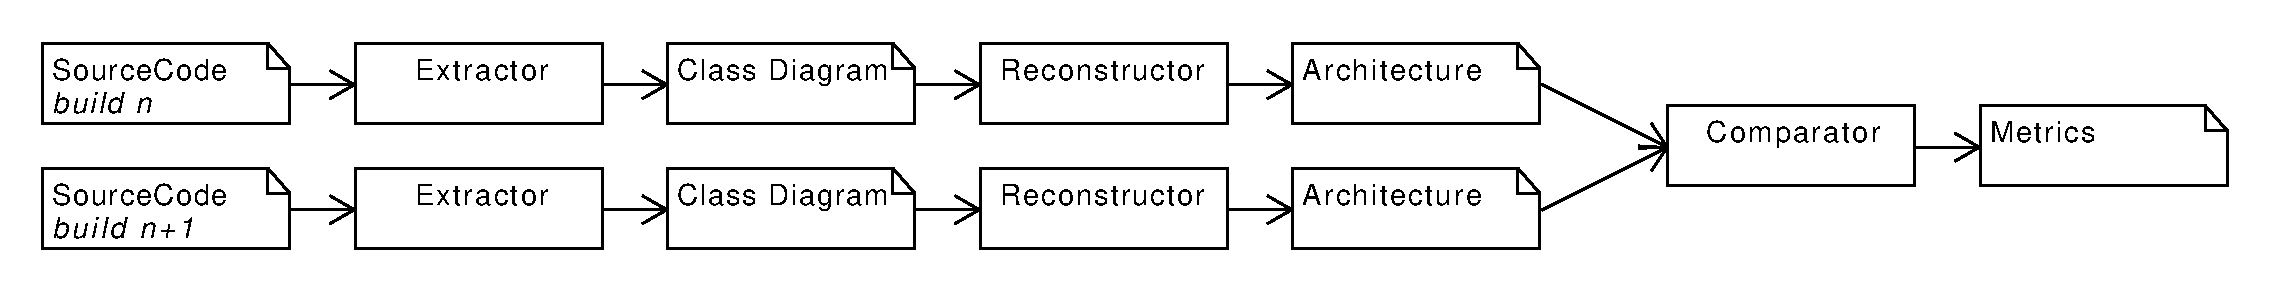
\includegraphics[width=7in]{assets/overview.pdf}
	\caption{Overview of the process~\sn{I still find figures 1 and 2 confusing.. there is a relationship between them but some things are not consistent.. Can you unify this in one figure with clearer steps and then modify the text description accordingly?}}
	\label{overview}
\end{figure*}

\begin{table}
	\caption{Ten Largest Projects under Study}
	\label{tableProjects}
	\centering
	\scalebox{0.9}{
	\begin{tabular}{ | c | c | c | c | c | }
		\hline
		project name & commits & analyzed & range & project type \\
		\hline
		sonarqube & 11590 & 4573 & 1.25y & Code Analyzer \\
		graylog2-server & 8490 & 842 & 4.25y & Log Analyzer \\
		okhttp & 5367 & 1770 & 3.5y & HTTP Client \\
		cloudify & 4984 & 821 & 2.5y & Dev. Framework \\
		structr & 3809 & 1253 & 2.5y & Development App \\
		owlapi & 3238 & 2178 & 3.5y & OWL API \\
		jOOQ & 3196 & 451 & 3y & SQL API \\
		checkstyle & 3029 & 325 & 2y & Code Analyzer \\
		vectorz & 3025 & 46 & 3.5y & Math Library \\
		owner & 2671 & 2099 & 3.5y & Property Files API \\
		\hline
	\end{tabular}
	}
\end{table}


In this study, we have analyzed $159$ projects from the TravisTorrent dataset, which use Java and Maven. In the dataset are $241$ projects which use Java as their main programming language and are built with Maven. We excluded projects, which do not have pushed anything to the master branch or only have one commit, because we cannot compare architectures if there is only one. Then there are some projects where builds or logs could not be retrieved anymore from GitHub and TravisCI or the toolchain was unable to reconstruct the architecture. We are left with $49,531$ commits. An exemplary list of the ten biggest analyzed projects, in terms of unrestricted commits, can be found in table \ref{tableProjects}.

As described, we see failures at or before compilation as a source of build failures. 
Vassallo et al. \cite{CIFailTypes} classified the different fail types based on Maven goals. Because it is inefficient for us to rerun every build we analyzed for multiple goals, we will use a simpler approach. Furthermore, because some builds are already older and have dependencies which are not anymore available or need to be installed manually, the approach to rerun everything may even be impossible. Still, we base our heuristic on the Maven goals.
Hence, we analyze the log files from TravisCI for all builds, to classify the build outcome further, than in success and failure. We used a heuristic to filter first lines that start with the ``\texttt{[Error]}'' keyword, which is used by the Maven log to indicate defects. Afterwards, we look for ``Compilation failure'', ``dependencies'' or ``test failures'' to categorize the failures. We map this with the actual build result to mitigate errors in the heuristic, so that only if the actual build failed, we use one the fail categories. We end up with five possible build results: (0) no error, (1) error during dependency resolution, (2) compilation failure, (3) test failure or (4) unknown error. 

Because the build tool impacts the outcome of the build but not the architecture itself \cite{FailsCorr}, we will limit the study to only one build tool. Although this introduces bias, it ensures consistent results in return. HUSACCT needs the path to the source files, so we can exclude test files and resources. Therefore, we choose the build tool maven with its convention over configuration paradigm. In this way we can be sure where everything is stored in the file structure. This eases the implementation of the class structure extraction. 
Because there are possibly multiple builds for the same commit, we only use the build that builds a certain version of the software first. The following builds are most likely only configuration changes of the CI server and do not introduce new change. Thus, we can ensure that changing configuration does not bias the results. Instead, we compare the changing source code based on the older configuration, i.e. the configuration which is equal to the one of the older build. 

In general, to get an architectural change, we have to follow three steps. First, we need to extract the class structure out of the source code, then we reconstruct the architecture and eventually we take two architectures and compare them with each other to get a change metric (Fig. \ref{overview}). 
The complete source code and results can be found in our GitHub repository.\footnote{\url{https://github.com/jodokae/cmput663-architecture}}

\subsection{Framework}

\begin{figure}[!t]
	\centering
	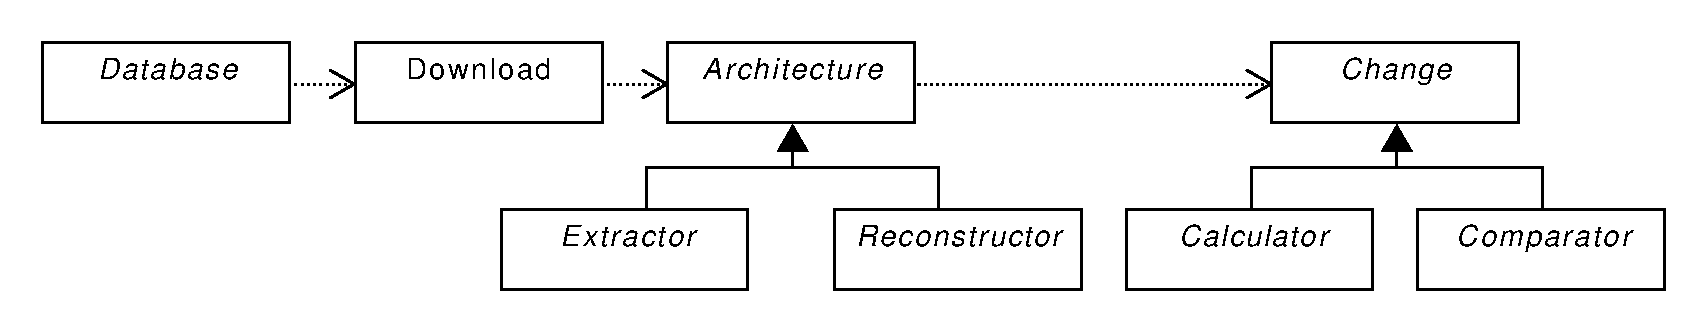
\includegraphics[width=3.45in]{assets/architecture.pdf}
	\caption{Structure of the Framework~\sn{see my comments about improving this diagram.. In general, it needs to be clear the input/output of each process and the order.. For example, extractor and reconstructor appear as parallel things while it seems that one uses the output of the other.. If you want to indicate they are part of the same step, you can put a bigger dotted box around them for instance}}
	\label{frameworkStructure}
\end{figure}

We implement a framework to extract the considered architectural change metrics between two commits of a given project.~\sn{Which language is this implemented in and provide link to github repo.. this link can also be provided in the beginning of the section once we settle on the final structure}
Figure \ref{frameworkStructure} shows an overview of the structure of our framework.
 
\paragraph{Step 1} extracts the unique commit ID of each CI build from the TravisTorrent database~\sn{please say TravisTorrent in the box instead of "Database".. also differentiate between process/step boxes and input/output sources.. right now, all are boxes but the boxes mean different things. Maybe also use Step 1, Step 2 etc. in the figure. For a process, use nouns "Repo Downloader" etc. or verbs "Download Repo" .. the important thing is to be consistent and to use meaningful names}.

\paragraph{Step 2} uses the commit ID extracted in step 1 to download a snapshot of the project from GitHub.


\paragraph{Step 3} extracts the architecture information needed to compare two commits in the next step. 
Specifically, Step 3 is split into two parts, (a) the extraction of the class structure and (b) the reconstruction of the architecture. 

In Step 3a, we use the extractor of the HUSACCT framework~\cite{todo} to extract relation triples in the form of relationship type, source, target (see listing \ref{lst1:rsf}), and save this information in the Rigi Standard Format (rsf) \cite{RSF}, because the ARCADE tools rely on this format. This relational system is easy convertible into a graph structure or a database and stores the modules implicitly in the dependencies. ~\sn{I don't understand the next part about the downside. please elaborate} The downside of this format is that the modules cannot be extracted separately but only implicitly while analyzing the dependencies. Fortunately, this is irrelevant for our work. For simplicity, and because it is not used in the further analyses~\sn{if it is not used in further analysis, why do you extract it?}, the dependency types are restricted to ``subPkg'', ``contains'' and ``references'', where ``subPkg'' means \todo{...}, ``contains'' means that that a package contains a Java type, and ``references'' is any dependency between two Java types. The results are then fed into the reconstruction.

\begin{figure}[!t]
	\centering
	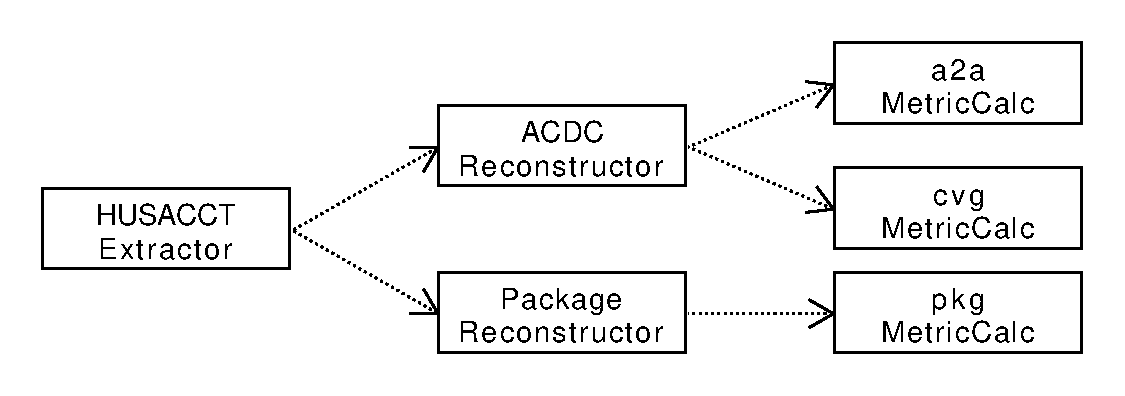
\includegraphics[width=3.45in]{assets/implementedArc.pdf}
	\caption{Implemented tool chain}
	\label{implToolchain}
\end{figure}

\begin{lstlisting}[
frame = single, 
belowskip=-0.8 \baselineskip,
float,
caption=Rigi Standard Format example~\sn{maybe have a references relation there too?},
label=lst1:rsf,
columns=flexible
]
subPkg   checkstyle checkstyle.grammars
subPkg   checkstyle checkstyle.gui
contains checkstyle checkstyle.Main
\end{lstlisting}

\begin{table*}
	\caption{Metrics}
	\label{tableMetric}
	\centering
	\begin{tabular}{ | c | l | l | c |  }
		\hline
		Name & Full Name & Description & Builds With Change \\
		\hline
		\#V & Number of Vertexes & Number of changing modules & 1.6\%  \\
		\#E & Number of Edges & Number of changing dependencies & 3.6\% \\
		A. Inst & Absolute Instability & Change of instability for weighted dependencies & 16\% \\
		R. Inst & Relative Instability & Change of instability for unweighted dependencies & 3.4\% \\
		deg & Average node degree & Sum of Edges (unweighted) per module & 3.1\% \\
		a2a & architecture to architecture & number of steps to get from one architecture to another & 67\% \\
		$\text{cvg}_\text{src}$ & cluster coverage (source) & \% of changed modules based on the earlier arch & 39\% \\
		$\text{cvg}_\text{tar}$ & cluster coverage (target) & \% of changed modules based on the latter arch & 40\% \\
		\hline
	\end{tabular}
\end{table*}


In Step 3b, we reconstruct the architecture of the current version of the system based on the information extracted in Step 3a. We implement~\sn{implement or use?} two different architecture reconstruction techniques.

The first is ACDC, because it has one of the best reconstruction accuracy rates when compared to other commonly used techniques \cite{arcRec-comparison}. 
While an implementation of ACDC is provided in the ARCADE framework, this implementation works directly on the Java byte code.  Given that a common reason for failing builds (here:~\sn{what is "here"? Can't you cite previous work?} $10\%$ of the builds) is compilation errors, it is thus better if we can instead use directly the source code for extracting the architecture. This is why we have Step 3a where we extract the class structure using the source-based HUSACCT extractor, and then feed that information into ACDC after deactivating its own first level extraction.~\sn{you don't really re-implement it then.. it is just a minor modification right?}

The second reconstruction technique is package reconstruction, which is often used as ground truth analysis~\sn{cite source? and also why do we need two techniques ?}.
This technique looks for the root packages in the system. If there are only a few root packages, it is assumed that the implemented architecture lies a level deeper in the packages. For example, if there is only the ``org.sonar'' as root, this is just the base container and not an architectural element. Therefore, all direct children of this package are considered as modules until there are at least an acceptable number of modules. In this work, we consider 10 as the minimum amount of modules needed. This number was chosen with manual sampling over different projects, so that the achieved results were the most consistent with the believed~\sn{believed? by who?} intended architecture. We follow Song et al.'s approach of considering all ``references'' edges as dependencies~\cite{ArcAsGraph}. ~\sn{it is not clear.. did you implement this yourself? Make that clear}

\paragraph{Step 4} calculates the architectural changes between two given commits.
As explained in Section \ref{sec:Metrics}, we use the ARCADE metrics a2a and cvg as well as Martin's metrics. We calculate the ARCADE metrics on the architecture extracted by ACDC. Cvg is calculated twice, one based on the modules of the first version (called \textit{source}) and one based on the second version (called \textit{target}).
The coupling metrics are calculated on the package architecture to have some ground truth metrics for comparison. We calculate five package metrics~\sn{first time these package metrics are mentioned? what's the relation to Section 3?}; thus, we have 8 metrics in total summarized in Table \ref{tableMetric}.
For every module, the absolute number of incoming and outgoing edges are calculated, the degree of the node (sum over ingoing and outgoing edges), as well as the absolute and relative instability. The absolute instability is based on the absolute number of connections between the modules, i.e. if Module A has only three ingoing connections from Module B, then the afferent coupling is considered three. For the relative instability, the coupling is instead considered one~\sn{why is it considered one?}, so it is not measured how tightly connected two modules are, just if they are connected at all.

Since we need to calculate the change for the complete architecture, and not for each module, we calculate the mean instabilities and node degree as well as the absolute number of modules (vertexes) and dependencies (edges).

We then perform a pairwise comparison of each metric. To compare proportional metrics, like instability, the difference between the values is taken, e. g. if architecture A has an average instability of $30\%$, and architecture B has an average instability of $25\%$, then they are $5\%$ different to each other (Equation \ref{eq:relDiff}). For metrics with absolute numbers, like node degree, the similarity is the proportion of the two values, e.g. A has an average node degree of $8$ and B has $10$, then they are $80\%$ similar, i.e. $20\%$ change (Equation \ref{eq:absDiff}).

\begin{equation} \label{eq:relDiff}
c_{rel}(m_1, m_2) =  \min\{m1, m2\} - \max\{m1, m2\}
\end{equation} 

\begin{equation} \label{eq:absDiff}
	c_{abs}(m_1, m_2) = 1 - \frac{\min\{m1, m2\}}{\max\{m1, m2\}}
\end{equation} 


\sn{moved here temporarily till I figure out where it belongs}
Then, for every two subsequent commits, we compare the architectures and save the results in a JSON file. With the methodology structured into this framework, the research can easily be expanded with more reconstructors or metric calculators. Therefore, one needs only to implement a new subclass for the changing module, store its result in the Rigi Standard Format and it can be integrated with all existing tools. Doing so, we have combined HUSACCT and ACDC and integrated it with the ARCADE metrics. Similarly, we have implemented the package reconstruction and metrics, so that both ways of computing change can be run independent or simultaneous (Fig. \ref{implToolchain}).

\subsection{Evaluation}

The calculated metrics are tested for correlation with the build result. This is done in multiple ways. First, the metric is tested against the direct build outcome, then the previous or following $b$ outcomes for $b \in \{2, 3, 5, 10\}$. This means we look for correlation between change in build $x$ and the build result in the builds $\{x, x \pm 1, \hdots, x \pm b\}$. From this, we can see if architectural change correlates to build failures in recent history or near future. 
Because we have different types of failures, for testing in the near past and future, the fail types get categorized into non-failure and failure. In this way, we get a single integer how many builds failed, instead of having multiple variables. 
Then, every metric is converted to a Boolean, which is true if there is a change and false if there is none. This is calculated with a threshold $t$, where everything below $t$ is considered to be no change, and anything above as a change for $t \in \{0.01, 0.02, 0.03, 0.04, 0.05, 0.1, 0.2, 0.5\}$. These values were chosen because most found changes in the dataset were small (Fig. \ref{fig:histograms}) We take these thresholds to find out if small changes affect the amount correlation present in the data. Every comparison which includes no Boolean variables is run with Pearson's correlation test, the others with Spearman's test. 

\begin{figure*}[!t]
	\centering
	\begin{subfigure}{2.3in}
		\centering
		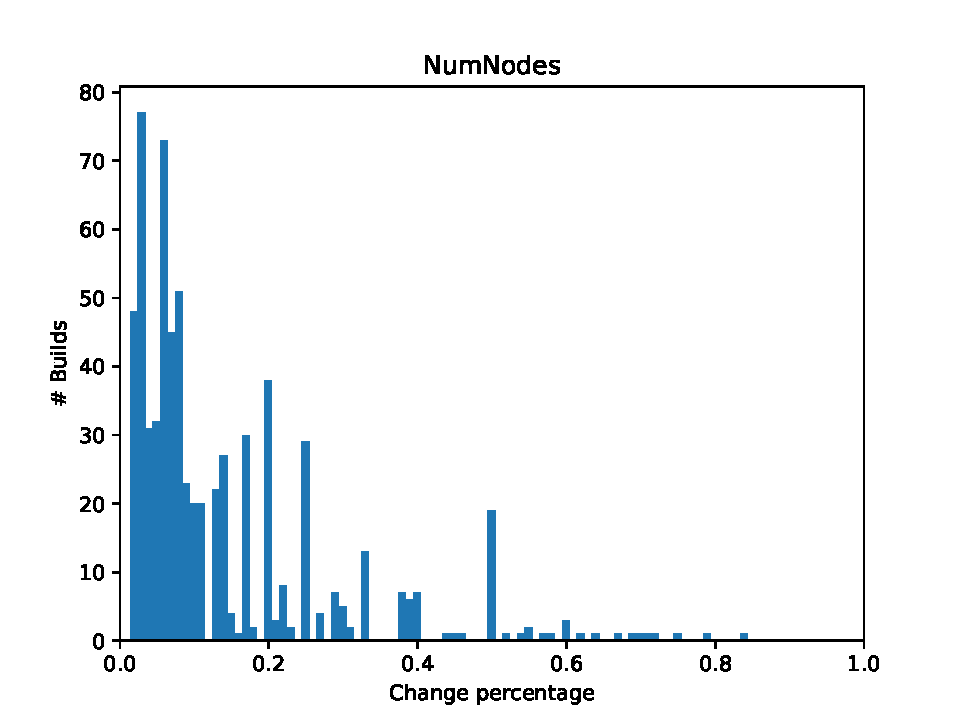
\includegraphics[width=2.3in]{assets/NumNodes.pdf}
		\caption{\#V}
		\label{numNodesHist}
	\end{subfigure}%
	\begin{subfigure}{2.3in}
		\centering
		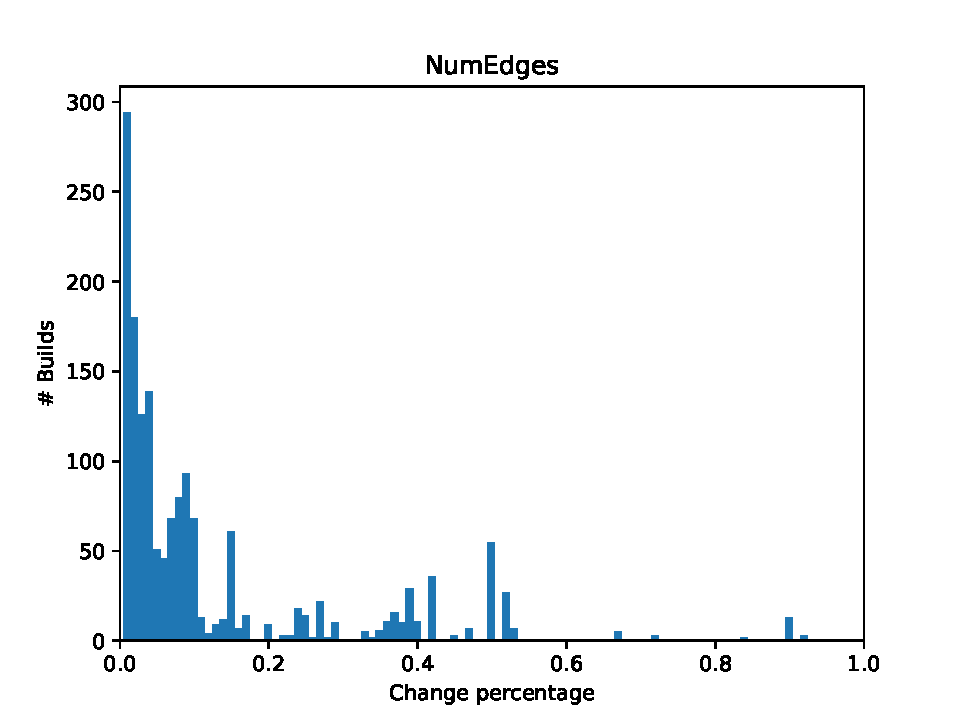
\includegraphics[width=2.3in]{assets/NumEdges.pdf}
		\caption{\#E}
		\label{numEdgesHist}
	\end{subfigure}%
	\begin{subfigure}{2.3in}
		\centering
		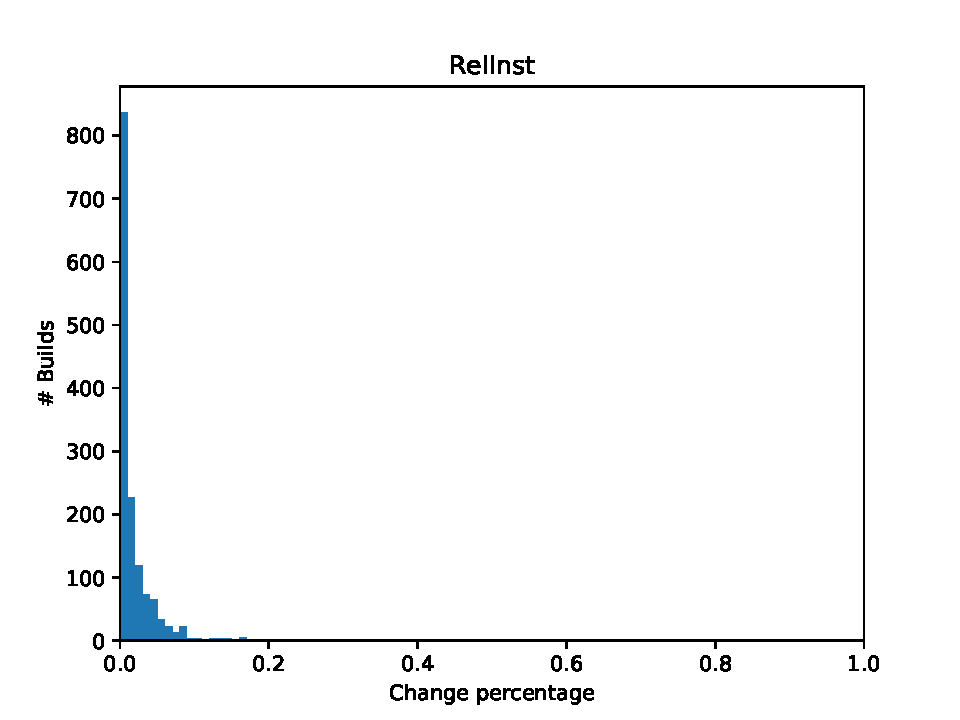
\includegraphics[width=2.3in]{assets/RelInst.pdf}
		\caption{rel. Inst}
		\label{relInstHist}
	\end{subfigure}
	\begin{subfigure}{2.3in}
		\centering
		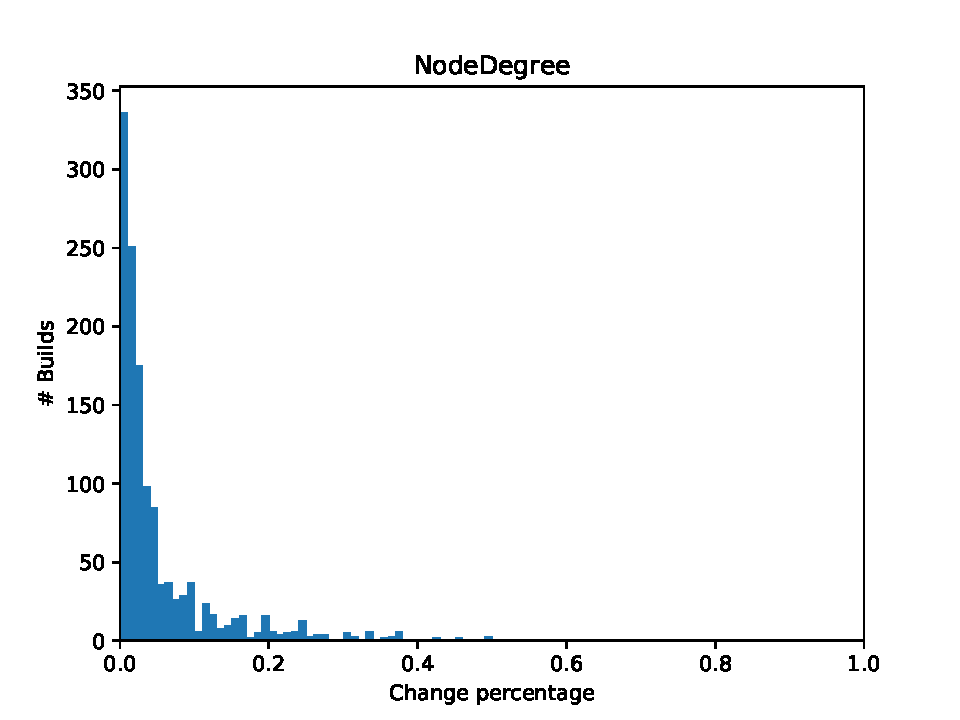
\includegraphics[width=2.3in]{assets/NodeDegree.pdf}
		\caption{deg(V)}
		\label{nodDegHist}
	\end{subfigure}%
	\begin{subfigure}{2.3in}
		\centering
		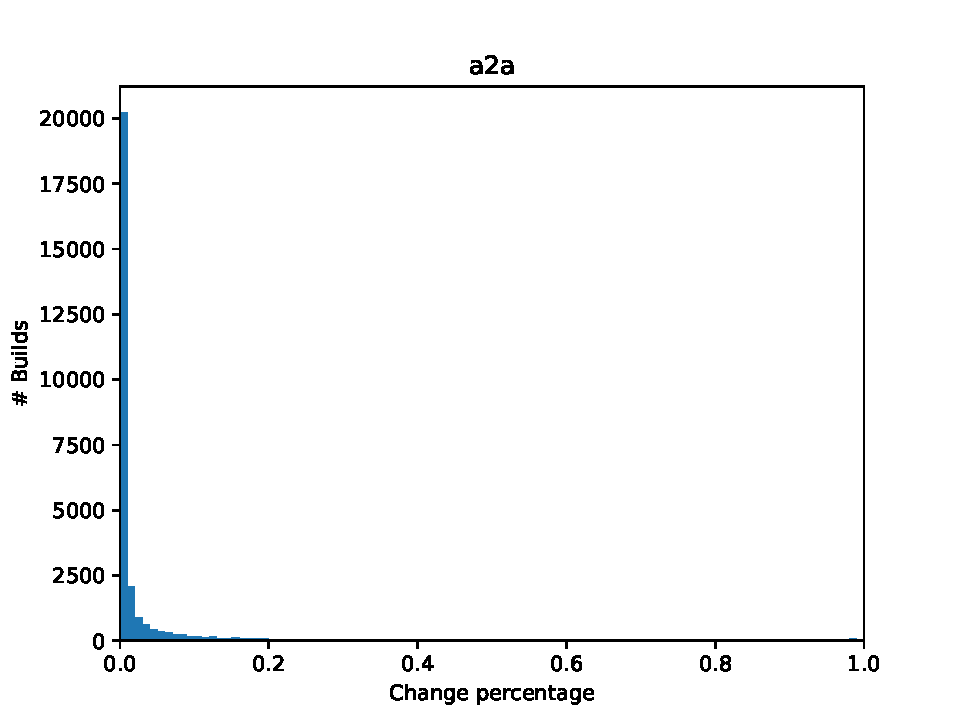
\includegraphics[width=2.3in]{assets/a2a.pdf}
		\caption{a2a}
		\label{a2aHist}
	\end{subfigure}%
	\begin{subfigure}{2.3in}
		\centering
		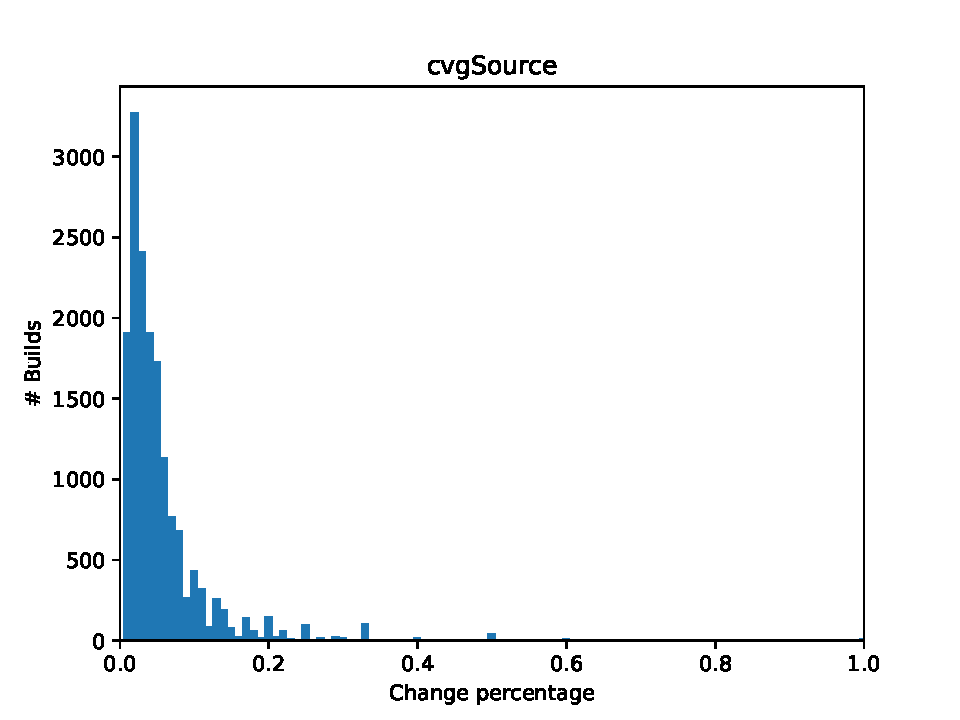
\includegraphics[width=2.3in]{assets/cvgSource.pdf}
		\caption{cvg src}
		\label{cvgHist}
	\end{subfigure}
	\caption{Histograms metric over all projects}
	\label{fig:histograms}
	
\end{figure*}

\section{Results}

This section presents the findings with the proposed methodology. First, the projects under study are introduced, then calculated metrics are evaluated and, eventually, the correlation between the metrics and the build outcomes is shown.

\subsection{Studied Projects}

We have studied $49,531$ commits from $159$ projects which use Java Maven. The pass rate is $84.9\%$. Around $10\%$ of the builds failed because of errors before or during the compilation of the software. On third of the errors could be mapped to test errors. The remaining part of the fails were not further separated, but are for example configuration errors or wrong used maven plugins.
The active time of the projects varies. For the ten biggest projects (in terms of number of commits) it is between one and four years of development time, some start at a well-established state (the TravisTorrent dataset starts, for example, at build number 500 for SonarQube), others at build 1 (e.g. Checkstyle). The projects vary in their application field. In the ten biggest projects, there are two code analyzers, three APIs, a web client and an IDE, some for databases, linear algebra or ontologies. Table \ref{tableProjects} gives a detailed list.

\subsection{Metric Evaluation}

p values are all 0 

\begin{table}
	\scalebox{0.85}{
	\begin{tabular}{ | c | c | c | c | c | c | c | c | c | }
		\hline
		& \#V & \#E & A. Inst & R. Inst & deg & a2a & cvg src & cvg tar \\
		\hline
		\#V & 1 & 0.93 & 0.58 & 0.59 & 0.69 & 0.23 & 0.45 & 0.49 \\
		\#E & 0.93 & 1 & 0.63 & 0.71 & 0.83 & 0.25 & 0.51 & 0.55 \\
		A. Inst & 0.58 & 0.63 & 1 & 0.81 & 0.43 & 0.2 & 0.44 & 0.46 \\
		R. Inst & 0.59 & 0.71 & 0.81 & 1 & 0.56 & 0.22 & 0.48 & 0.52 \\
		deg & 0.69 & 0.83 & 0.43 & 0.56 & 1 & 0.18 & 0.41 & 0.46 \\
		a2a & 0.23 & 0.25 & 0.2 & 0.22 & 0.18 & 1 & 0.38 & 0.37 \\
		cvg src & 0.45 & 0.51 & 0.44 & 0.48 & 0.41 & 0.38 & 1 & 0.91 \\
		cvg tar & 0.49 & 0.55 & 0.46 & 0.52 & 0.46 & 0.37 & 0.91 & 1 \\
		\hline
	\end{tabular}
	}
\end{table}


We have extracted 8 architecture change metrics. Most builds show no change (table \ref{tableMetric}). This is to be expected, since most changes in the system should not be architectural changes. 
Only a2a has more changing builds than non-changing builds. But then, most of these changes are really small, as shown in Fig. \ref{a2aHist}. In other metrics, most changes are quite small as well, with only few big architectural changes (Fig. \ref{cvgHist} and \ref{numEdgesHist}). This seems usual, because we assume that the architecture does not have big changes that often. Only the number of nodes (Fig. \ref{numNodesHist}) has more widespread changes, which lies in the nature of the reconstruction process. Because a minimum number of ten nodes per architecture is hard coded into the package-architecture reconstruction, but is done level wise, a change from ten to nine nodes cannot appear, but will result in a change from 10 to 18 nodes. The effects of this red line are not as bad as they sound, because the node degree and number of edges metrics are in the expected norm, so that it is indicated that the few outliers do not affect the results badly.


In table \ref{tableMetricCorr} the correlation between the metrics is shown. All p values were equal or close to 0. the highest p value cross-metric wise is $3.7^{-102}$. 
The package metrics are highly correlated, all with c values above $0.6$ up to $0.92$. a2a does not correlate with the other metrics strongly, only between $0.10-0.17$, while cvg shows low to medium correlation to the package metrics. 
Still, this gives the indication that all metrics are truly an indicator for architectural change if we assume that at least one of them is, since the p-values do not leave any doubt, that the metrics are dependent.
As expected, the metrics look at disjunct types of architectural change, a2a and cvg highlight the change at the module level, whereat the Martin's metrics take the focus at the relationship between the modules. This strengthens our confidence in the chosen tool chain. 


\subsection{Relationship}

Around $16\%$ of all builds that had architectural change failed ($P(f|c)$). This we found while extracting data for all metrics for all tested change thresholds, at the median. The values ranged from $8-18\%$. 
If we check for the probability of change under the condition that the build failed ($P(c|f)$), we get a range from $0\%$ up to $60\%$. For the package metrics, the probability was almost always low, but the the ARCADE metrics, the results are more interesting. First, the probability drastically decreases while the change threshold increases. If we look at the probability of architectural change according to the a2a metric, and we consider every change, then we end up with $61\%$.. Of course, this is natural since we do not change the number of failing builds but the number of considered changes when we change the threshold of what we consider a change. 
Constant values around $p(f|c) = 16\%$ and peak values for $p(c|f)$ with $61\%$ for a2a and $35-36\%$ for cvg, leads us to the possibility that there is also some correlation between the data.

\subsection{Correlation}

%TODO Maybe make table with all values
%TODO Manual Sampling - Check some values

When we first analyzed only the ten biggest projects, we found lot of correlation values between $0.1\%$ and $3\%$, with even some values as high as $11\%$. Now, when analyzing all projects, the feeling, that there is no correlation gets confirmed. When calculating correlation between architectural change and the different types of build outcome, some of the metrics show no correlation at all ($c < 0.4\%$ and $p > 0.25$), while the top metrics, a2a and cvg, peak at $4.3\%$ ($p = 6.8 \cdot 10^{-22}$) and $3.0\%$ ($p=1.2 \cdot 10^{-11}$). 
The threshold that controls how many previous or following builds were considered, had no large impact. Only when going really high, so it considers more than $40$ previous builds, it was possible to see a significant rise in the correlation (Fig. \ref{a2aPrevN}). But first, a rise from $3\%$ to $6\%$, although it is a doubling, is not that interesting, and second to consider the previous $80$ builds, where the peak occurred, is more by chance than by actual correlation. In other words, it is improbable that code that was committed $80$ builds before the current one, influences the architecture. 
Nevertheless, we computed the correlation values over the next $80$ builds for different change thresholds, and confirmed this educated feeling that the correlation is even lower than the one for the next $10$ builds after the initial peak.
The highest correlation found for a2a was the one with a change threshold of $0.0$, i.e. every little change was considered as change. But even the best correlation, in a realistic scenario, was only $4\%$ over the next ten builds (Fig. \ref{a2aPlot}). 

Some of the metrics have low p-values which shows that there is a statistical significant relationship between build outcome and those metrics. But this correlation is so small that we cannot conclude this as a meaningful impact. Because taking the smallest changes into consideration increases the correlation coefficient, and the threshold for previous and following builds had no big significant change on that coefficient, it must be assumed that the stronger correlations could be noise. Because the strongest correlation was found with the a2a metric, which works on the modules and not the relationship between them, the possible correlation is at the modules and within them. Furthermore, over all correlations, the tendency was towards a positive value, with $38\%$ negative correlation values. This shows, if there truly is a correlation, then change is occurring more often around non failing builds, whereas a static architecture shows in the near of failing builds. 

\begin{figure}[!t]
	\centering
	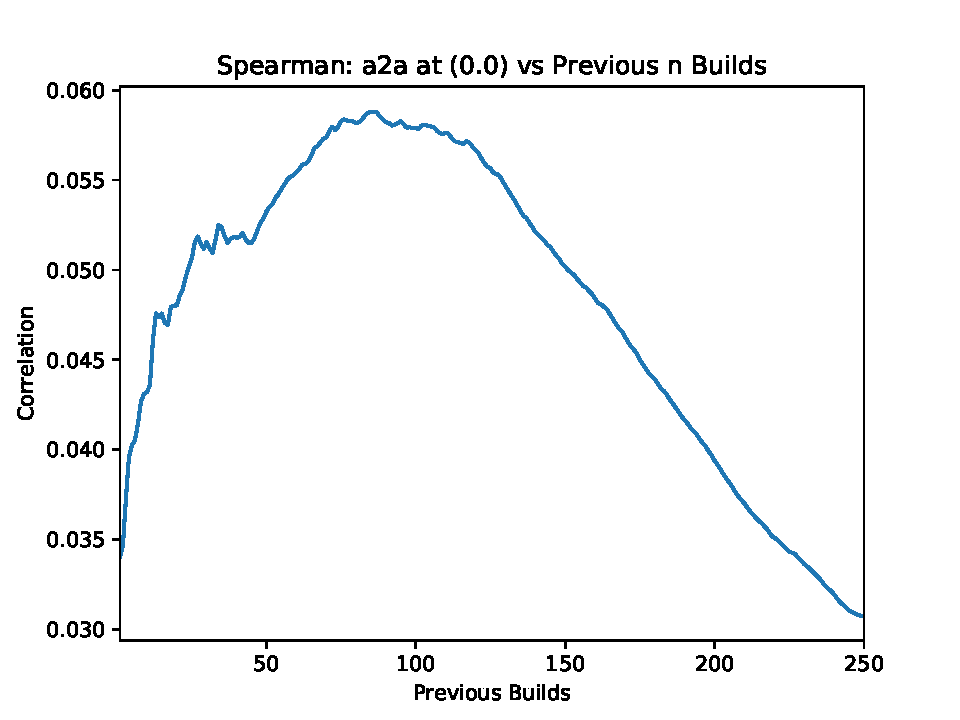
\includegraphics[width=3in]{assets/PrevN}
	\caption{a2a vs previous n builds over 0.0 threshold }
	\label{a2aPrevN}
\end{figure}

\begin{figure}[!t]
	\centering
	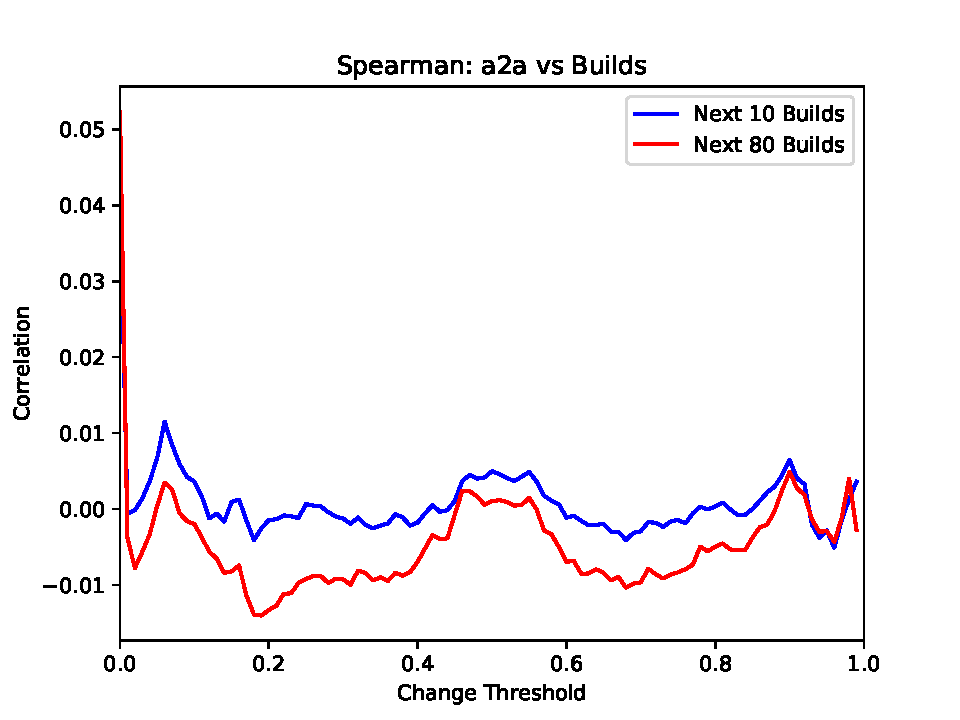
\includegraphics[width=3in]{assets/a2aCorr}
	\caption{a2a vs next ten and eighty builds over different change thresholds }
	\label{a2aPlot}
\end{figure}


\section{Discussion}

While checking $159$ Java projects, no significant correlation between architectural change and build results was found. Apart from there actually being no correlation, there could be various factors influencing this result. 

First of all, only Java projects which are build with Maven were evaluated. Hence, we cannot conclude our results globally to Java or other programming languages. Still, we believe that our results are not dependent to Maven, and can be obtained with other build tools, as well. 

Despite having projects which start at build one, the number of failing builds was relatively small. 
It is possible that the missing connection between architecture and build results lies in the possibility that the big projects which have a stronger impact on the results have a well thought-through architecture and do not change it in a problematic way.
This can be backed up by the fact that most found changes are below a threshold of $10\%$ change. It would be interesting to see if projects with a more unstable architecture show more failures. We have not found interesting cross-project differences.

It is also possible, that the problems which are produced by architectural change are not transferred into build results but to a different level, e.g. (1) code coverage or (2) number failed tests. Unfortunately, the dataset does not give the opportunity to check for those, because they are (1) not reported and (b) have missing values in around $20\%$ of the builds. The fact that software architecture is important is common knowledge. We showed that it changes over the lifetime of a project. However, it remains unknown how architecture change affects the progress of the development process.

As Garcia et al. \cite{arcRec-comparison} show even the best recovery techniques have problems detecting the true architecture. Therefore, it is possible that HUSACCT and ARCADE are not the right tools for the research question. This problem was addressed since we consider multiple recovery techniques and rely on studies which evaluate ARCADE as being one of the most accurate recovery tools. The produced metrics highly correlate, which strengthens the claim that the change detection is working as intended. Still, it is possible that the chosen metrics are not the best set. Because they correlate so strongly, they are a weak feature set if one would try to use machine learning techniques to predict the build outcome. For this, a broader set of metrics is necessary. 

In the future, more metrics and extractors should be added to the framework. Then, it is necessary to broaden the research to find better quantitative data which show problems in the software that could be caused by bad or changing architecture. Because this work introduces an easy expandable framework, this should be possible with little to no effort.

\section{Conclusion}

While analyzing $49,531$ builds from $159$ different Java Maven projects from various domains, we could not find any significant impact of architectural change on build outcome.
We approached this result through an easily expandable framework to recover the architecture from the builds using one extractor, two reconstructors, and three metric sets based on previous researches. In total, $8$ metrics were tested for correlation in $6$ different scenarios including the previous and following builds. 

The hypothesis that architectural change impacts CI build outcomes at or near the change was rejected. The highest correlation found was around $4\%$ and would imply that change leads to fewer failures. This could just be noise, due to the well-established nature of the studied projects, or that is no correlation between architectural change and build outcome. 

We conclude that change does not impact the build outcome and, thus, the research questions have to be changed. Since it is known that the architecture impacts the development, other quantitative features must be found to measure the impact. We propose to extend the measured metrics, because we believe that one metric cannot explain the impact alone, and search for correlation in more nonfunctional metrics, like code coverage or development pace.
The built framework can be efficiently adapted for the new questions through extracting more facts out of the code using various tools. 

\bibliographystyle{ACM-Reference-Format}
\bibliography{literature}

\end{document}
\grid
